\graphicspath{{appendices/}}

\chapter{Example settings file}
\makeatletter\@mkboth{}{Appendix}\makeatother
\label{appen:settings}
\begin{figure}[H]
    \centering
    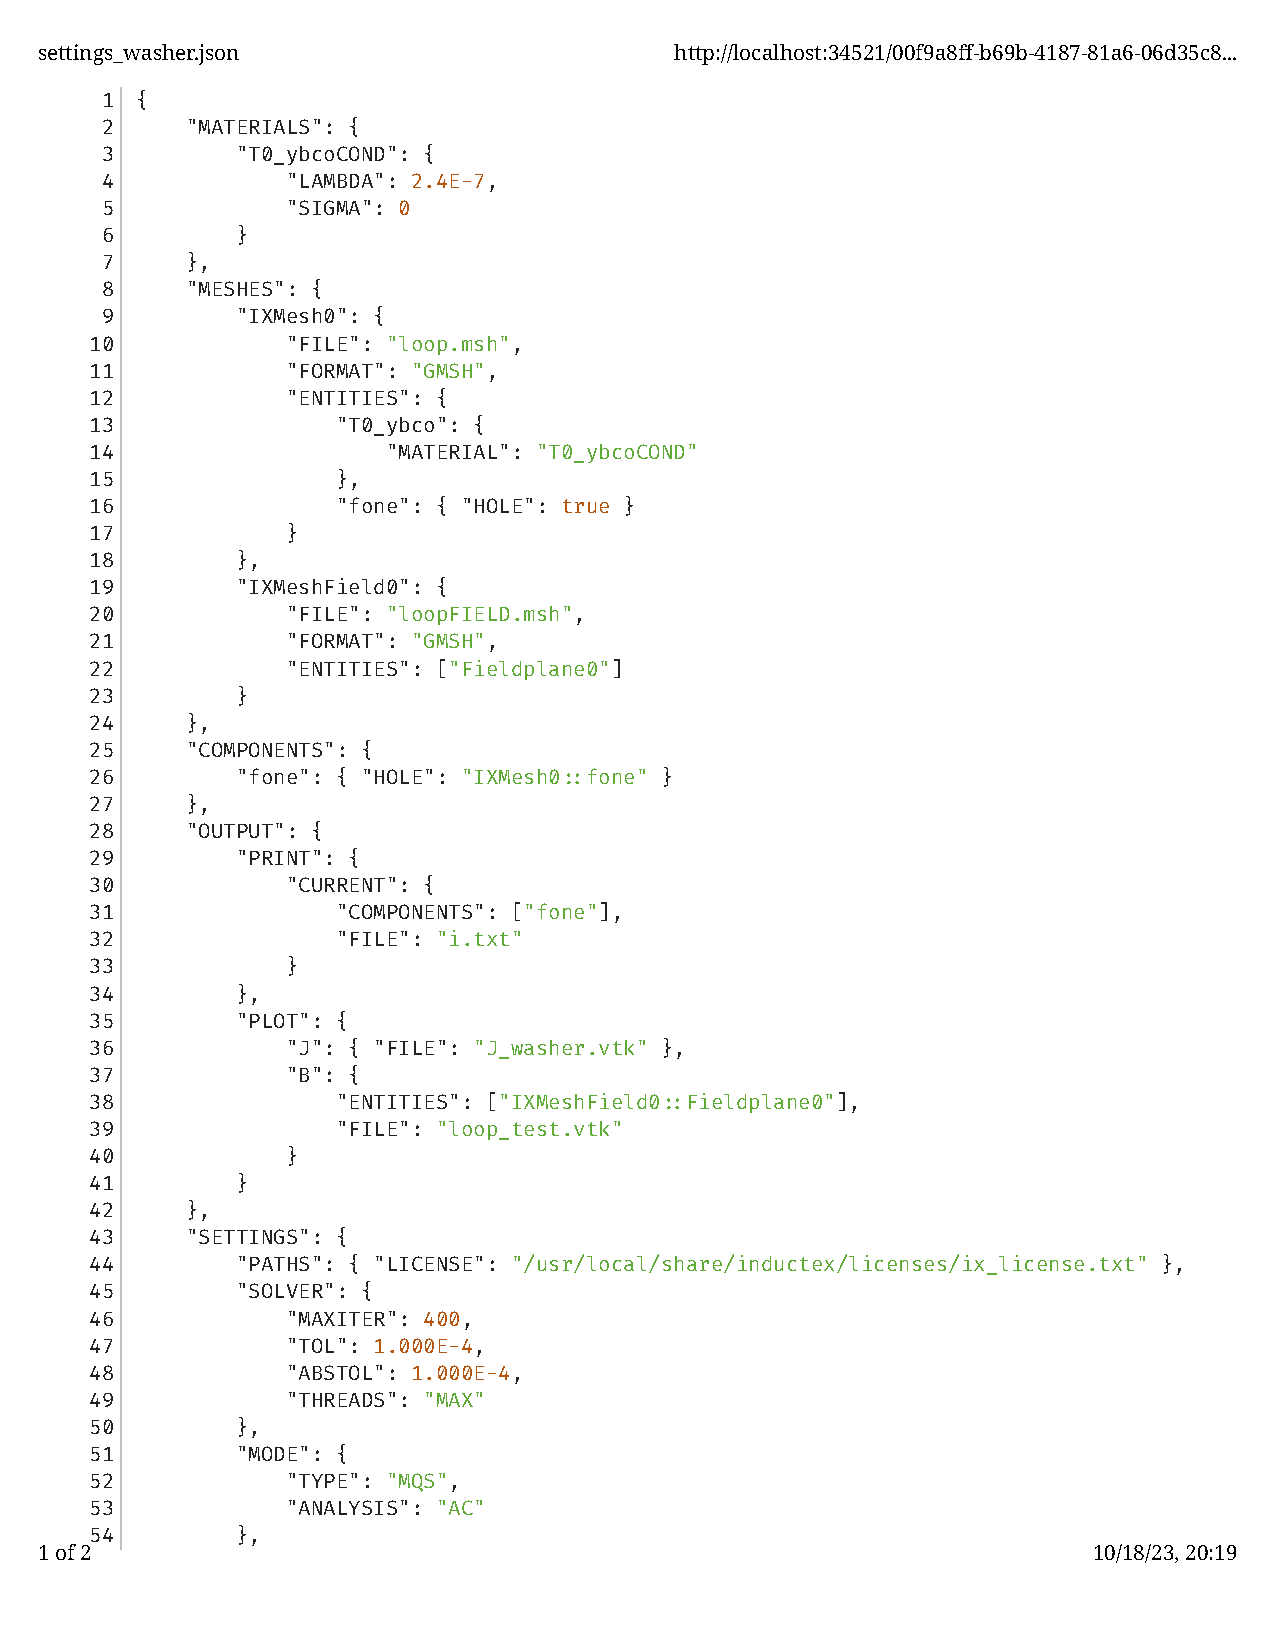
\includegraphics[width=0.9\textwidth]{settings.pdf}
    \label{fig:sett1}
\end{figure}
\newpage
\begin{figure}[H]
    \centering
    \includegraphics[width=0.9\textwidth,page=2]{settings.pdf}
    \label{fig:sett2}
\end{figure}

\chapter{Project Planning Schedule}
\makeatletter\@mkboth{}{Appendix}\makeatother
\label{appen:PPS}

\begin{table}[H]
    \centering
    \begin{tabular}{lll}
        \hline
        \textbf{Task Name}                                   & \textbf{Start Date} & \textbf{Due Date} \\ \hline
        Skripsie Admin                                       & 06/28/2023          & 06/30/2023        \\
        Read Feynmann lectures volume III                    & 07/01/2023          & 07/20/2023        \\
        Read S.M. Anton's PhD thesis                         & 07/21/2023          & 08/07/2023        \\
        Complete and submit GA plan                           & 08/08/2023          & 08/09/2023        \\
        Develop, Implement and test noise extraction module  & 08/10/2023          & 09/03/2023        \\
        Develop, Implement and test mesh optimisation module & 09/04/2023          & 09/23/2023        \\
        Determine Lit review topics                          & 08/10/2023          & 08/12/2023        \\
        Write first 3 sections of lit review                 & 08/13/2023          & 09/02/2023        \\
        write the last three sections of lit review              & 09/03/2023          & 09/23/2023        \\
        write design section                                 & 09/24/2023          & 10/07/2023        \\
        obtain results for results section                   & 09/24/2023          & 10/11/2023        \\
        write results section                                & 10/12/2023          & 10/22/2023        \\
        write introduction                                   & 10/18/2023          & 10/20/2023        \\
        submit preliminary report                            & 10/21/2023          & 10/21/2023        \\
        Make changes to report as recommended by supervisor  & 10/23/2023          & 10/29/2023        \\
        Spelling and grammar checks                          & 10/31/2023          & 10/31/2023        \\
        Write abstract                                       & 10/30/2023          & 10/30/2023        \\
        Create poster and video                              & 11/01/2023          & 11/04/2023        \\
        final check and submission                           & 11/05/2023          & 11/05/2023        \\
        final submission due                                 & 11/05/2023          & 11/06/2023        \\ \hline
        \end{tabular}
        \caption{The project planning schedule}
        \label{tab:pps}
    \end{table}


\chapter{Outcomes Compliance}
\makeatletter\@mkboth{}{Appendix}\makeatother
\label{appen:OC}

\section{GA 1. Problem Solving}
This project required the implementation of an algorithm to calculate the expected noise power in a SQUID. It extends on previous works by generalizing existing techniques to work on any geometry. The algorithm converts a complex 3-dimensional mesh into a single number. The task does not have a defined solution and requires solving many individual problems including but not limited to numerically calculating a surface integral, electromagnetic simulation with TetraHenry, mesh optimisation and modelling of superconducting structures. The details of these challenges are discussed in Chapter \ref{chap:nex} and \ref{chap:meshopt}.

\section{GA 2. Application of Scientific and Engineering Knowledge}
The topic relied on a good understanding of scientific and engineering concepts introduced in my undergraduate years as well as the application of this knowledge to solve open-ended problems. It required knowledge of calculus, vector calculus, electromagnetism, and programming. Along with topics introduced in the undergraduate years, a rudimentary understanding of quantum mechanics and superconductors was needed. Chapters \ref{chap:litreview} and \ref{chap:solutiondevelopment} show the fulfilment of these outcomes.
\section{GA 3. Engineering Design}
The problem statement was very open-ended and required refinement (Chapter \ref{chap:dgoals}). System design techniques were used to solve the engineering design problem in Chapter \ref{chap:high level design}. Once the problem was formally defined it was broken down into smaller sub-problems in Chapter \ref{chap:ddesign}. Solving the sub-problems required drawing knowledge from a wide variety of sources about the topics listed in GA 2.
\section{GA 4. Investigations, experiments and data analysis}
Once the system was implemented an investigation was performed to determine the validity of the results. This required using previous results obtained by simulation as well as physical tests and comparing them to results obtained from my system. The system was tested for accuracy (how closely the output of my system when operating on a previously solved problem matches the true solution) and performance. The testing procedure was designed and then implemented using Python. The regex and OS modules were used to perform parameter sweeps and automate testing. The data output from this testing procedure was analysed to extract conclusions about the performance and accuracy of the system. This achievement of this outcome is demonstrated in Chapter \ref{chap:results}. 
\section{GA 5. Engineering methods, skills and tools, including Information Technology}
To perform the data analysis required as mentioned in GA 4 jupyter notebooks were used in conjunction with the numpy, pandas, matlpotlib and seaborn libraries. The results of this analysis are shown in \ref{chap:results}. Electromagnetic simulations were done with TetraHenry and InductEx. CMake and VCPKG were used to manage compilation and code dependencies. Knowledge of the CLion IDE was crucial to the implementation of this project. GitHub and Git were used for project backup and source control. To model the 3D SQUID structures they had to be created with GMSH. This was done using the GMSH scripting language. Evidence of the above can be found in the GitHub repository \cite{paulcode}. ParaView was used to quickly visualise the results generated by TetraHenry. To improve personal productivity Trello was used to track active tasks as well as future tasks.

\section{GA 6. Professional and technical communication}
The project includes a written report and an oral presentation. These demonstrate competence to communicate effectively, both orally and in writing. Communication with my supervisor included progress reports both as presentations and demonstrations of work progress.

\section{GA 8. Individual work}
I was solely responsible for the completion of my project with little to no input from others. 

\section{GA 9. Independent Learning Ability}
The project required an understanding of complex topics not previously encountered by me. The broad topic gave no context to the required knowledge for the successful completion of the project. Chapter \ref{chap:litreview} demonstrates the process through which I acquired the necessary knowledge. It explores the topics needed to grasp the problem in the order by which they were encountered by me.  